% AE496 UGP: conference paper (IEEE format), condensed from report.tex.
% Every number here is taken from report.tex, which is checked against the runs
% by experiments/verify_report.py. Check this file with
%     python experiments/check_paper_numbers.py
% Build:  cd report && pdflatex paper.tex && pdflatex paper.tex
\documentclass[conference]{IEEEtran}

\usepackage{cite}
\usepackage{amsmath}
\usepackage{graphicx}
\usepackage{booktabs}
\usepackage{balance}
\usepackage[hidelinks]{hyperref}

\graphicspath{{../figures/}}

\newcommand{\Rey}{\mathrm{Re}}
\newcommand{\St}{\mathrm{St}}
\newcommand{\Cd}{C_d}

\begin{document}

\title{Predicting Vortex Shedding Behind a Circular Cylinder with
Physics-Informed Neural Networks}

\author{\IEEEauthorblockN{Peeyush Agarwal}
\IEEEauthorblockA{Department of Aerospace Engineering\\
Indian Institute of Technology Kanpur\\
Kanpur, India}}

\maketitle

\begin{abstract}
Physics-informed neural networks (PINNs) trained without data on the unsteady
wake of a circular cylinder tend toward the steady symmetric solution, which
satisfies the Navier--Stokes equations exactly. We study this failure at
$\Rey = 100$ using lattice Boltzmann reference data validated against Qu et
al.\ ($\St$ within $0.04\%$, $\Cd$ $3.5\%$ high). Averaged over four start
phases and five seeds, a data-free PINN retains 31.1\% of the reference wake
amplitude. Causal time-marching raises this to 56.4\%, but at equal training
budget it adds only 7.7 points. Combining marching with random Fourier
features and a Reynolds decomposition gives 72.9\%, between 70\% and 77\% at
every start phase, at a relative $L_2$ error of 0.031. This configuration
predicts one shedding period from physics alone, but over five periods it
sheds 10.4\% slow and ends about half a cycle out of phase. Holding the phase
requires 350 supervised points per period taken from the predicted span, which
turns the task into reconstruction from sparse measurements. The gain from
the combined strategies holds for $\Rey = 60$--$180$. A recurrent sequence
PINN does not replace marching. For data-driven forecasting, a physics
residual makes a Fourier neural operator worse on the validated data; on an
earlier, harder dataset it helps the operator at short horizons, but not a
U-Net or a convolutional GRU.
\end{abstract}

\begin{IEEEkeywords}
physics-informed neural networks, vortex shedding, causal training, lattice
Boltzmann method, Fourier neural operator
\end{IEEEkeywords}

\section{Introduction}

Above $\Rey \approx 47$ the wake of a circular cylinder sheds a K\'arm\'an
vortex street at a frequency given by the Strouhal number $\St = fD/U$.
Predicting this flow with a data-free PINN is difficult for three reasons. The
steady symmetric field satisfies the equations and boundary conditions exactly,
so it is an easily reached minimum of the residual loss. Networks learn low
frequencies first (spectral bias), which works against an oscillatory wake.
The initial condition is a single time slice and is weakly weighted against the
residual over the space--time domain.

Chuang and Barba~\cite{chuang2023} found that a data-free PINN behaves like a
steady solver, and Shah~\cite{shah2026}, on a confined cylinder benchmark,
found that only supervised combinations of training techniques escape this
collapse. Causal training, either by time-marching~\cite{krishnapriyan2021} or
by causal weighting~\cite{wang2024causality}, has been shown to help on
one-dimensional problems, but neither of these cylinder studies tests hard
time-window marching. Separately, Renn et al.~\cite{renn2023} forecast
cylinder wakes with a purely data-driven Fourier neural operator
(FNO)~\cite{li2021fno}.

The objective of this work is to reproduce the PINN collapse on validated
reference data, to identify which training strategy prevents it under a
controlled comparison, and to test whether adding physics to an operator
forecast improves it. Here, prediction means computing the flow beyond the
data the model is given; the reference data are otherwise used only for
scoring. The contributions are an unsteady Navier--Stokes operator for the
\texttt{underPINN} framework~\cite{underpinn}, a validated lattice Boltzmann
dataset, a phase-averaged ablation with equal-budget controls, and a
comparison of physics-informed forecasting across three operator backbones.

\section{Reference Data}
\label{sec:lbm}

The reference wake is computed with a D2Q9 two-relaxation-time lattice
Boltzmann solver written in JAX, with half-way bounce-back on the cylinder and
free-slip lateral walls. The inlet is $25D$ upstream of the cylinder in a
domain $60D$ long. The production run uses $\Rey = 100$, $D = 24$ lattice
units, $\mathrm{Ma} = 0.087$, a $1440 \times 1200$ grid and $2\%$ blockage. It
records 641 snapshots over 20 shedding periods on a $241 \times 121$ grid
($\Delta x = 0.083D$, $\Delta t^{*} = 0.19$). Table~\ref{tab:validation}
compares it with Qu et al.~\cite{qu2013}.

\begin{table}[!t]
\centering
\caption{Validation at $\Rey = 100$ against Qu et al.~\cite{qu2013}}
\label{tab:validation}
\begin{tabular}{lccc}
\toprule
Quantity & Present & Benchmark range & Error \\
\midrule
Mean drag $\Cd$       & 1.3634 & 1.318--1.336 & $+3.5\%$ \\
Strouhal number $\St$ & 0.1648 & 0.164--0.166 & $-0.04\%$ \\
R.m.s.\ lift $C_l'$   & 0.2362 & 0.222--0.235 & $+6.2\%$ \\
\bottomrule
\multicolumn{4}{p{0.92\columnwidth}}{\footnotesize Errors are relative to
their values $\Cd = 1.317$, $\St = 0.1649$ and $C_l' = 0.2224$; the range is
their compilation of eight studies.}
\end{tabular}
\end{table}

\subsection{Validation of the Reference Solution}

Two corrections were needed. First, the free-slip walls reflect sound, so the
domain behaves as an acoustic duct with a transverse mode at $\St_a = 0.1155$.
Without treatment the wake locks onto this mode over long records
($\St = 0.1132$ over 38 periods). An absorbing layer of $8D$ at each wall that
relaxes the populations toward the free-stream equilibrium removes it.
Blevins~\cite{blevins1985} showed experimentally that a transverse acoustic
wave can shift cylinder shedding to its own frequency. Second, at $D = 32$,
moving the inlet from $8D$ to $25D$ upstream lowers $\Cd$ by $4.7\%$, from
$+7.4\%$ to $+2.3\%$ against Qu et al., and takes $\St$ from $+3.0\%$ to
$+0.3\%$; the domain height has a much smaller effect. The grid is converged
at $D = 32$. The production value $D = 24$ reads $\Cd$ about $1.4\%$ high and
is kept so that the snapshot spacing matches PIV-like resolution. None of the
PINN or operator results depend on $\Cd$.

\section{Methodology}
\label{sec:method}

\subsection{Unsteady Navier--Stokes Operator}

The network maps $(x, y, t) \mapsto (u, v, p)$ and is trained on the
non-dimensional incompressible equations
\begin{align}
u_x + v_y &= 0, \\
u_t + u u_x + v u_y + p_x - \tfrac{1}{\Rey}(u_{xx} + u_{yy}) &= 0, \\
v_t + u v_x + v v_y + p_y - \tfrac{1}{\Rey}(v_{xx} + v_{yy}) &= 0.
\end{align}
\texttt{underPINN} provides only a steady residual, so an unsteady operator was
implemented, with derivatives computed by forward-mode automatic
differentiation. It annihilates the Taylor--Green vortex to
$1.6\times 10^{-16}$, matches a reference Hessian implementation to
$2.8\times 10^{-17}$, and reduces to the framework's steady residual to
$5.6\times 10^{-17}$.

\subsection{Training Strategies}

The baseline is a multilayer perceptron $[3, 128^{\times 6}, 3]$ trained for
$20\,000$ epochs on the equation residual, boundary conditions and initial
condition over one shedding period, with no data other than the initial
condition. Three strategies are added as independent switches on the same
trainer:
\begin{itemize}
  \item \emph{Fourier features}~\cite{tancik2020}, against spectral bias. The
        bandwidth is $\sigma = 8$, except in the phase-0 ablation and the
        supervision study, which use $\sigma = 2$.
  \item \emph{Reynolds decomposition} $u = u_0 + u'$, where the mean $u_0$ is
        a separate frozen network fitted to the measured mean.
  \item \emph{Causal time-marching}: four windows of a quarter period solved
        in sequence, each taking its initial condition from the previous
        window's network. The run uses ground truth only once.
\end{itemize}
The combination of all three is denoted \texttt{all}.

\subsection{Evaluation Protocol}

The main metric is \emph{shedding retained}: the ratio of transverse-velocity
r.m.s.\ at a wake probe between the PINN and the reference. A value near 0\%
means collapse to steady flow. Field accuracy is the relative $L_2$ error of
the velocity field. Because retention depends on the phase of the cycle at
which a run starts, the main comparison is averaged over four start phases
with five seeds each. A marched run trains four windows, so each marched
configuration is also compared with a single-window run given the same
$80\,000$ epochs.

\section{Results}
\label{sec:results}

\subsection{Baseline PINN}

The baseline retains between 19.0\% and 43.2\% of the wake depending on the
start phase, 31.1\% on average (Table~\ref{tab:phase}). Training for
$80\,000$ epochs raises the mean to 48.6\% but leaves the dependence on start
phase in place.

\begin{table}[!t]
\centering
\caption{Shedding Retained by Start Phase (Five Seeds Each)}
\label{tab:phase}
\setlength{\tabcolsep}{4pt}
\begin{tabular}{lcccccc}
\toprule
Configuration & 0 & $\tfrac14$ & $\tfrac12$ & $\tfrac34$ & Mean & $L_2$ \\
\midrule
Baseline     & 43.2\% & 20.3\% & 42.1\% & 19.0\% & 31.1\% & 0.166 \\
Marching     & 70.6\% & 40.4\% & 73.8\% & 40.7\% & 56.4\% & 0.156 \\
\texttt{all} & 74.9\% & 70.2\% & 76.6\% & 70.0\% & \textbf{72.9\%} & \textbf{0.031} \\
\bottomrule
\end{tabular}
\end{table}

\begin{figure}[!t]
\centering
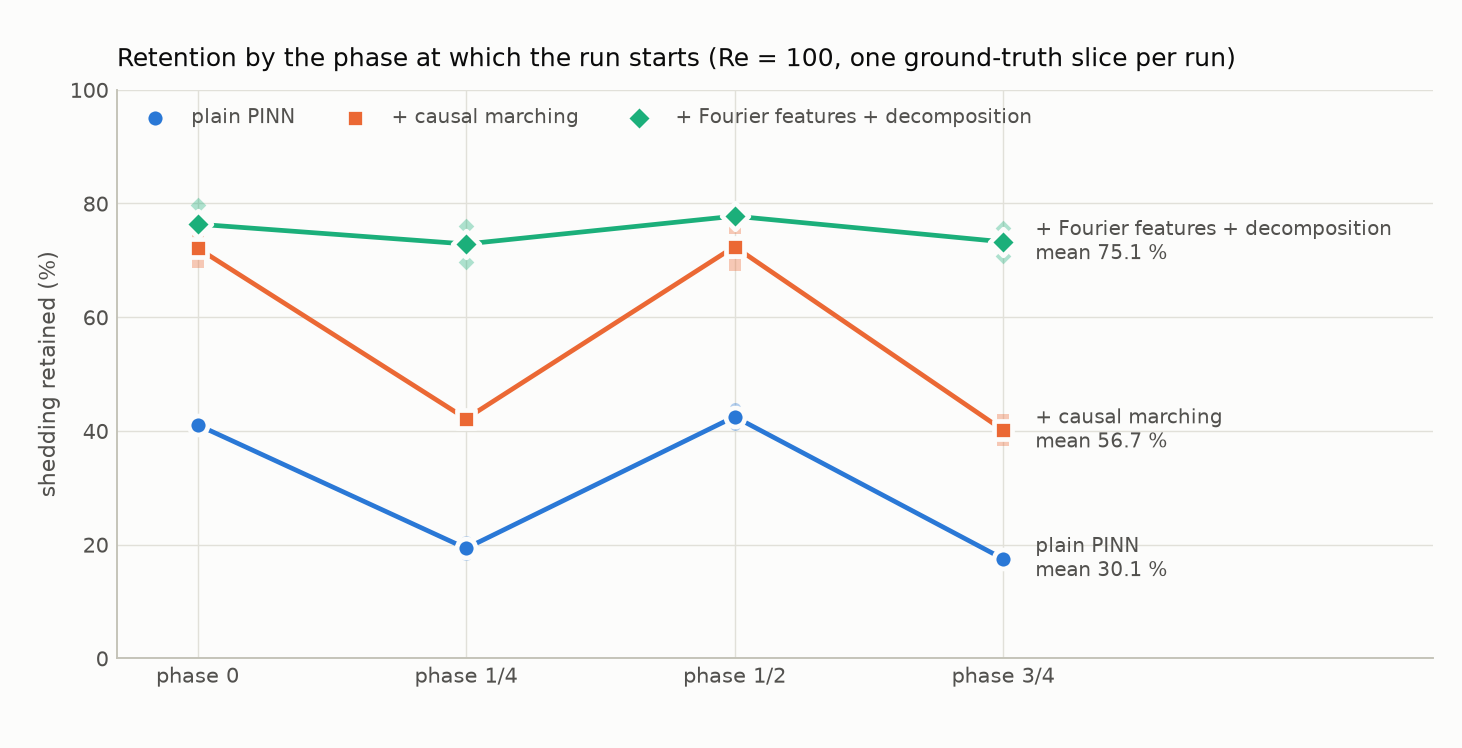
\includegraphics[width=\columnwidth]{phase.png}
\caption{Shedding retained by start phase, all runs.}
\label{fig:phase}
\end{figure}

\subsection{Ablation of Training Strategies}

In a phase-0 ablation (two seeds), Fourier features (36.9\%) and the Reynolds
decomposition (36.1\%) each retain slightly less than the baseline (41.1\%),
although the decomposition halves the field error. Marching raises retention
at every start phase, from 31.1\% to 56.4\% on average, but keeps the
baseline's dependence on start phase. Only the combination of all three is
insensitive to start phase, at a fifth of the field error of either
alternative (Table~\ref{tab:phase}, Fig.~\ref{fig:phase}). The 95\% intervals
over seeds are $\pm 1.5$, $\pm 0.9$ and $\pm 4.6$ points for the three rows.

Table~\ref{tab:budget} separates the effect of marching from the extra
training it receives. Alone, marching beats an equal-budget single window by
7.7 points, less than the 17.5 points that longer training gives the baseline.
With Fourier features and the decomposition in place, marching adds 34.1
points and wins all 20 pairings. The strategies are therefore complementary,
in agreement with Shah~\cite{shah2026}. An earlier version of this study gave
each marched window a fresh reference snapshot; that raised retention at phase
0 to 93.0\% and 94.5\%, so about twenty points of the earlier result came from
extra ground truth.

\begin{table}[!t]
\centering
\caption{Marching Against Single-Window Runs of Equal Budget}
\label{tab:budget}
\setlength{\tabcolsep}{3pt}
\begin{tabular}{lcccc}
\toprule
Comparison & Marched & Single & Gain & Paired range \\
\midrule
Marching vs baseline   & 56.4\% & 48.6\% & $+7.7$  & $-2.2$ to $+15.8$ \\
\texttt{all} vs F+D    & 72.9\% & 38.7\% & $+34.1$ & $+20.0$ to $+55.2$ \\
\bottomrule
\multicolumn{5}{p{0.92\columnwidth}}{\footnotesize $80\,000$ epochs for both;
averaged over four start phases and five seeds; gains in points, paired by
phase and seed. F+D: Fourier features and Reynolds decomposition.}
\end{tabular}
\end{table}

\subsection{Prediction Horizon and Sparse Measurements}

Over one period, \texttt{all} matches the reference phase to $0.1^\circ$, at
73.5\% of its amplitude. Over five chained periods it keeps shedding, but at
$\St = 0.1476$, $10.4\%$ below the reference, and ends about half a cycle out
of phase (Fig.~\ref{fig:fields}); amplitude falls to 63.8\% and the field
error rises to 0.156. Data-free marching therefore predicts about one period
and sustains a wake beyond it, but does not hold the phase.

Measurements from inside the predicted span correct this. With supervised
points in every window (start phase 0, $\sigma = 2$, two seeds), 100 points
per window give 87.4\% retention and 500 give 96.9\%, with the field error
falling to 0.010. Table~\ref{tab:reanchor} gives selected rows of a sparse
re-anchoring study, in which $N$ supervised points are given to every $K$-th
window of the five-period chain and initial conditions stay chained. The phase
locks between 300 and 350 points per period: at 350 per period, 1\,750 points
in total and about 2\% of what per-window snapshots would use, both seeds hold
the phase to within 0.003 of a period and $\St$ to within 0.7\%. Because these
points lie inside the span being computed, this result is reconstruction from
sparse measurements, not forecasting.

\begin{table}[!t]
\centering
\caption{Sparse Re-Anchoring of the Five-Period Chain}
\label{tab:reanchor}
\setlength{\tabcolsep}{4pt}
\begin{tabular}{rrrrcc}
\toprule
$N$ & $K$ & Per period & Total & $\St$ error (\%) & Lag \\
\midrule
--- & --- & 0   & 0        & $-10.4$, $-10.2$ & 0.369, 0.345 \\
100 & 2   & 200 & 1\,000   & $-4.6$, $-3.3$   & 0.120, 0.100 \\
150 & 2   & 300 & 1\,500   & $-1.5$, $-1.3$   & 0.053, 0.042 \\
175 & 2   & 350 & 1\,750   & $-0.2$, $-0.7$   & 0.002, 0.002 \\
100 & 1   & 400 & 2\,000   & $-0.3$, $-0.2$   & 0.001, 0.001 \\
\bottomrule
\multicolumn{6}{p{0.92\columnwidth}}{\footnotesize Selected rows, two seeds
each. Lag is the cross-correlation lag over the last period, in shedding
periods, positive behind the reference.}
\end{tabular}
\end{table}

\begin{figure}[!t]
\centering
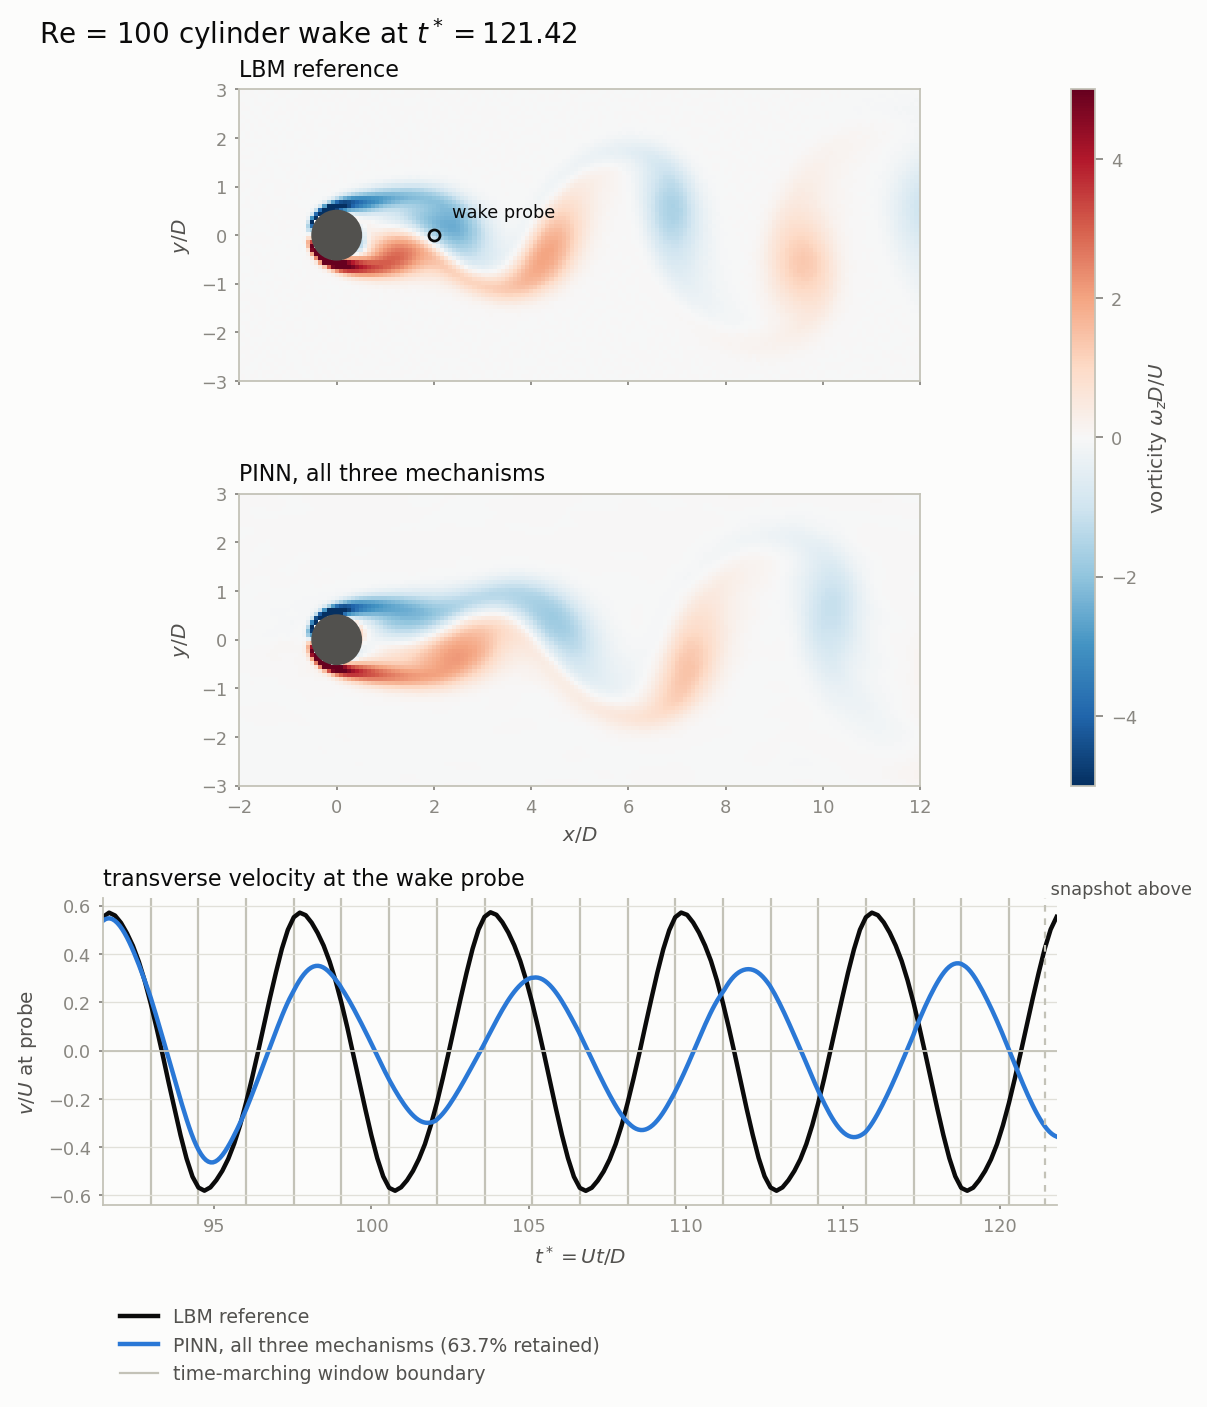
\includegraphics[width=0.9\columnwidth]{fields_v5.png}
\caption{Data-free \texttt{all} marched over five periods against the
reference. Top: vorticity at the end of the run. Bottom: transverse velocity
at the wake probe; grey lines are window boundaries.}
\label{fig:fields}
\end{figure}

\begin{figure*}[!t]
\centering
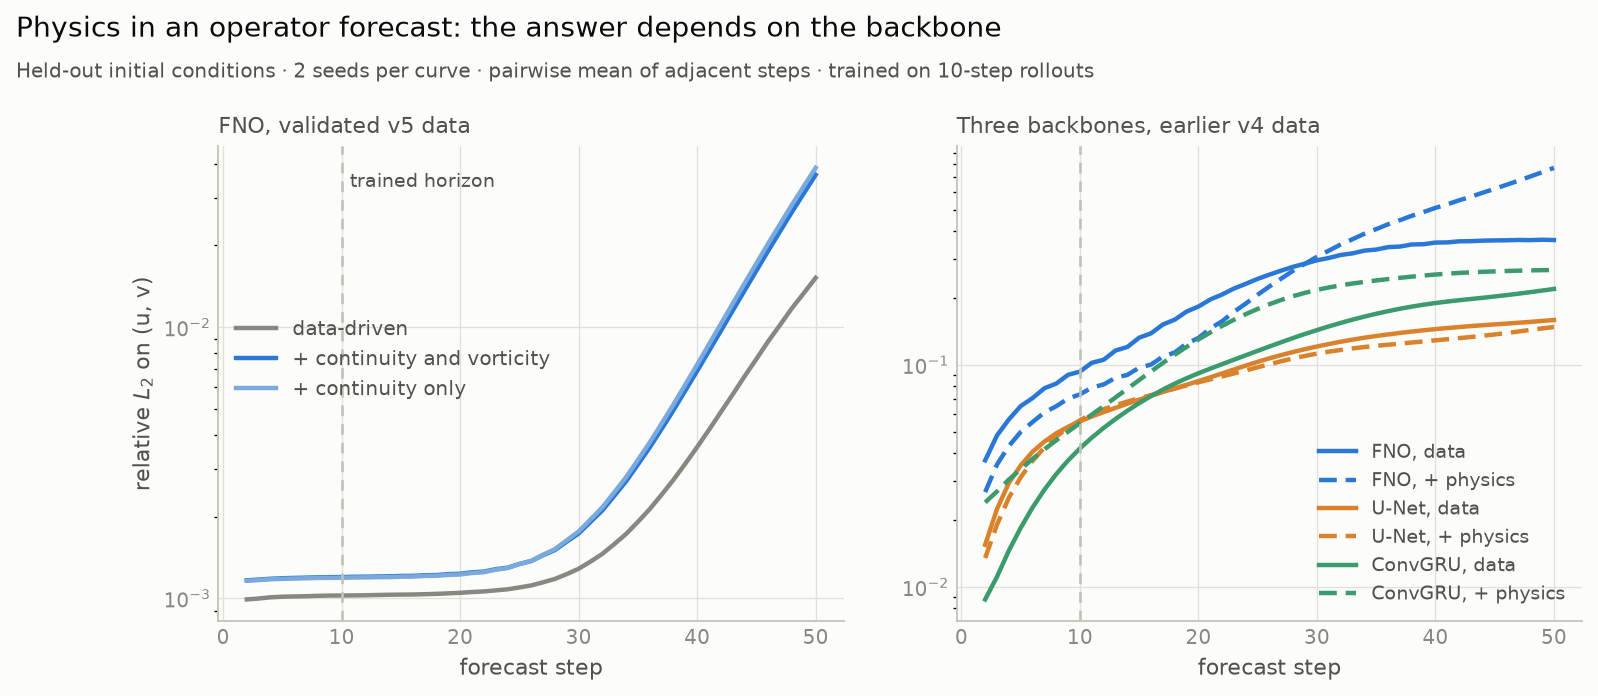
\includegraphics[width=0.72\textwidth]{operators.png}
\caption{Forecast error against horizon. Left: FNO on the validated dataset.
Right: three backbones on the earlier dataset, data-driven (solid) and with
physics (dashed).}
\label{fig:operators}
\end{figure*}

\subsection{Reynolds-Number Dependence}

The comparison was repeated at $\Rey = 60$--$180$, with new reference data at
each Reynolds number; the upper limit is set by the three-dimensional
transition at $\Rey_c = 188.5$~\cite{barkley1996}. Every dataset's $\St$ is
within $0.6\%$ of Qu et al. The baseline retains 24--45\% and \texttt{all}
63--79\%, and \texttt{all} reduces the field error from about 0.17 to
0.028--0.040 (Table~\ref{tab:resweep}). These runs use two seeds and a single
start phase, the beginning of each record, so the variation in the baseline
column reflects start phase and has no physical meaning. The insensitivity of
\texttt{all} to start phase was measured only at $\Rey = 100$.

\begin{table}[!t]
\centering
\caption{Data-Free Results Across Reynolds Number}
\label{tab:resweep}
\setlength{\tabcolsep}{3.5pt}
\begin{tabular}{lccccc}
\toprule
 & & \multicolumn{2}{c}{Shedding retained} & \multicolumn{2}{c}{$L_2$} \\
\cmidrule(lr){3-4}\cmidrule(lr){5-6}
$\Rey$ & $\St$ error & Baseline & \texttt{all} & Base. & \texttt{all} \\
\midrule
60  & $+0.51\%$ & 29.8, 33.5\% & 62.8, 69.1\% & 0.163 & 0.028 \\
80  & $+0.60\%$ & 40.2, 44.6\% & 75.5, 76.9\% & 0.173 & 0.028 \\
100 & $-0.04\%$ & 38.8, 41.5\% & 71.8, 78.5\% & 0.173 & 0.031 \\
120 & $+0.03\%$ & 23.9, 24.1\% & 71.5, 78.6\% & 0.170 & 0.036 \\
150 & $-0.28\%$ & 38.0, 41.4\% & 69.7, 75.1\% & 0.174 & 0.039 \\
180 & $-0.45\%$ & 24.1, 27.7\% & 77.5, 76.6\% & 0.171 & 0.040 \\
\bottomrule
\multicolumn{6}{p{0.92\columnwidth}}{\footnotesize $\St$ error is against Qu
et al.; retention for each of two seeds; $L_2$ is the two-seed mean.}
\end{tabular}
\end{table}

\subsection{Sequence Architectures}

PINNsFormer~\cite{zhao2024pinnsformer} and a GRU variant with the same
embedding were compared with the MLP. The GRU and MLP were run with two seeds
at all four start phases. On a single window the GRU retains 21.8\% against
the MLP's 30.1\%, and marched it retains 33.6\% against 56.7\%. PINNsFormer
was run once, at phase 0, because of its cost: on a single window it retains
34.9\% against the MLP's 40.4\%, and marched it reaches 77.5\% against
69.7\%, at 11.8 times the MLP's run time. Neither architecture prevents the
collapse without marching, and one marched run is not enough to show that
attention adds to it.

\subsection{Physics-Informed Operator Forecasting}

Following Renn et al.~\cite{renn2023}, an FNO maps two consecutive snapshots
to the next and is rolled out recursively. It trains on the first 70\% of the
record and forecasts from states in the last 30\%, so this is true
forecasting. A physics term is added through the vorticity-transport and
continuity residuals, which do not require pressure. On the validated dataset
the data-driven FNO reaches an error of 0.0010 at its trained horizon of ten
steps and 0.0152 after 50 steps, and the physics term makes it 16--18\% worse
at ten and twenty steps. Test states on this clean limit cycle are close to
the training data, which may explain why physics does not help.

On an earlier dataset whose fields contain the acoustic mode, and whose
held-out states are therefore less like the training data, physics lowers the
FNO error by 21\% at ten steps and 28\% at twenty, then crosses over at
0.8--1.0 shedding periods. Table~\ref{tab:backbones} repeats this test for a
U-Net~\cite{ronneberger2015} and a convolutional GRU~\cite{ren2022phycrnet}.
The physics term changes the U-Net error by at most 7\% and makes the ConvGRU
worse, so the short-horizon benefit is specific to the FNO
(Fig.~\ref{fig:operators}). Without physics, both convolutional networks
forecast better than the FNO, with 31 and 131 times fewer parameters.

\begin{table}[!t]
\centering
\caption{Forecast Error on the Earlier Dataset}
\label{tab:backbones}
\setlength{\tabcolsep}{2.6pt}
\begin{tabular}{lrcccccc}
\toprule
 & & \multicolumn{3}{c}{Data-driven error} & \multicolumn{3}{c}{Change with physics} \\
\cmidrule(lr){3-5}\cmidrule(lr){6-8}
Backbone & Params & 10 & 20 & 50 & 10 & 20 & 50 \\
\midrule
FNO     & 59.0\,M & 0.093 & 0.183 & 0.365 & $-21\%$ & $-28\%$ & $+111\%$ \\
U-Net   & 1.93\,M & 0.056 & 0.084 & 0.159 & $+1\%$  & $-1\%$  & $-7\%$ \\
ConvGRU & 0.45\,M & 0.042 & 0.092 & 0.220 & $+30\%$ & $+42\%$ & $+22\%$ \\
\bottomrule
\multicolumn{8}{p{0.92\columnwidth}}{\footnotesize Columns are forecast steps;
negative change is better. Two seeds.}
\end{tabular}
\end{table}


\section{Conclusion}

A data-free PINN retains 31.1\% of the cylinder wake at $\Rey = 100$, and the
amount depends on the start phase. No single strategy fixes this. Causal
time-marching adds only 7.7 points over an equal-budget baseline, but combined
with Fourier features and a Reynolds decomposition it retains 72.9\% on
average and between 70\% and 77\% at every start phase, at a field error of
0.031, with a similar gain across $\Rey = 60$--$180$. From physics alone, this
PINN predicts about one shedding period; over five it drifts in phase. About
350 supervised points per period from inside the predicted span hold the
phase, which is reconstruction rather than forecasting. Adding physics to an
operator forecast helped only the FNO, only at short horizons, and only on the
earlier dataset.

The main limitations are that most secondary studies use two seeds and
PINNsFormer was run once, that continuity between marching windows is enforced
only through the loss (exact enforcement~\cite{roy2024} is a possible next
step), and that the backbone comparison was run only on the earlier dataset.

\balance
\begin{thebibliography}{15}

\bibitem{chuang2023}
P.-Y. Chuang and L.~A. Barba, ``Predictive limitations of physics-informed
neural networks in vortex shedding,'' arXiv:2306.00230, 2023.

\bibitem{shah2026}
D.~Shah, ``Complementary, not cumulative: Interaction effects in
physics-informed neural networks for Navier--Stokes vortex shedding,''
arXiv:2608.19632, 2026.

\bibitem{krishnapriyan2021}
A.~S. Krishnapriyan, A.~Gholami, S.~Zhe, R.~M. Kirby, and M.~W. Mahoney,
``Characterizing possible failure modes in physics-informed neural networks,''
in \emph{Proc. Adv. Neural Inf. Process. Syst. (NeurIPS)}, 2021.

\bibitem{wang2024causality}
S.~Wang, S.~Sankaran, and P.~Perdikaris, ``Respecting causality is all you
need for training physics-informed neural networks,'' \emph{Comput. Methods
Appl. Mech. Eng.}, 2024, doi: 10.1016/j.cma.2024.116813.

\bibitem{renn2023}
P.~J. Renn, C.~Wang, S.~Lale, Z.~Li, A.~Anandkumar, and M.~Gharib,
``Forecasting subcritical cylinder wakes with Fourier neural operators,''
arXiv:2301.08290, 2023.

\bibitem{li2021fno}
Z.~Li, N.~Kovachki, K.~Azizzadenesheli, B.~Liu, K.~Bhattacharya, A.~Stuart,
and A.~Anandkumar, ``Fourier neural operator for parametric partial
differential equations,'' in \emph{Proc. Int. Conf. Learn. Represent.
(ICLR)}, 2021.

\bibitem{underpinn}
Aeroscience Computations and Analysis Lab, ``underPINN: A JAX framework for
physics-informed neural networks.'' [Online]. Available:
\url{https://github.com/Aeroscience-Computations-Analysis-Lab/underPINN}

\bibitem{qu2013}
L.~Qu, C.~Norberg, L.~Davidson, S.-H. Peng, and F.~Wang, ``Quantitative
numerical analysis of flow past a circular cylinder at Reynolds number between
50 and 200,'' \emph{J. Fluids Struct.}, vol.~39, pp.~347--370, 2013.

\bibitem{blevins1985}
R.~D. Blevins, ``The effect of sound on vortex shedding from cylinders,''
\emph{J. Fluid Mech.}, vol.~161, pp.~217--237, 1985.

\bibitem{tancik2020}
M.~Tancik \emph{et al.}, ``Fourier features let networks learn high frequency
functions in low dimensional domains,'' in \emph{Proc. Adv. Neural Inf.
Process. Syst. (NeurIPS)}, 2020.

\bibitem{barkley1996}
D.~Barkley and R.~D. Henderson, ``Three-dimensional Floquet stability analysis
of the wake of a circular cylinder,'' \emph{J. Fluid Mech.}, vol.~322,
pp.~215--241, 1996.

\bibitem{zhao2024pinnsformer}
Z.~Zhao, X.~Ding, and B.~A. Prakash, ``PINNsFormer: A transformer-based
framework for physics-informed neural networks,'' in \emph{Proc. Int. Conf.
Learn. Represent. (ICLR)}, 2024.

\bibitem{ronneberger2015}
O.~Ronneberger, P.~Fischer, and T.~Brox, ``U-Net: Convolutional networks for
biomedical image segmentation,'' in \emph{Proc. Med. Image Comput. Comput.
Assist. Interv. (MICCAI)}, LNCS vol.~9351, 2015, pp.~234--241.

\bibitem{ren2022phycrnet}
P.~Ren, C.~Rao, Y.~Liu, J.-X. Wang, and H.~Sun, ``PhyCRNet:
Physics-informed convolutional-recurrent network for solving spatiotemporal
PDEs,'' \emph{Comput. Methods Appl. Mech. Eng.}, vol.~389, Art.~no.~114399,
2022.

\bibitem{roy2024}
P.~Roy and S.~Castonguay, ``Exact enforcement of temporal continuity in
sequential physics-informed neural networks,'' arXiv:2403.03223, 2024.

\end{thebibliography}

\end{document}
